% ****** Start of file apssamp.tex ******
%
%   This file is part of the APS files in the REVTeX 4.1 distribution.
%   Version 4.1r of REVTeX, August 2010
%
%   Copyright (c) 2009, 2010 The American Physical Society.
%
%   See the REVTeX 4 README file for restrictions and more information.
%
% TeX'ing this file requires that you have AMS-LaTeX 2.0 installed
% as well as the rest of the prerequisites for REVTeX 4.1
%
% See the REVTeX 4 README file
% It also requires running BibTeX. The commands are as follows:
%
%  1)  latex apssamp.tex
%  2)  bibtex apssamp
%  3)  latex apssamp.tex
%  4)  latex apssamp.tex
%
\documentclass[%
 reprint,
%superscriptaddress,
%groupedaddress,
%unsortedaddress,
%runinaddress,
%frontmatterverbose,
%preprint,
%showpacs,preprintnumbers,
%nofootinbib,
%nobibnotes,
%bibnotes,
amsmath,amssymb,
%aps,
pra,
%prb,
%rmp,
%prstab,
%prstper,
%floatfix,
]{revtex4-1}

\usepackage{tabularx}
\usepackage{siunitx}
\sisetup{separate-uncertainty}
\usepackage{graphicx}% Include figure files
\usepackage{dcolumn}% Align table columns on decimal point
\usepackage{bm}% bold math
%\usepackage{hyperref}% add hypertext capabilities
%\usepackage[mathlines]{lineno}% Enable numbering of text and display math
%\linenumbers\relax % Commence numbering lines

%\usepackage[showframe,%Uncomment any one of the following lines to test
%%scale=0.7, marginratio={1:1, 2:3}, ignoreall,% default settings
%%text={7in,10in},centering,
%%margin=1.5in,
%%total={6.5in,8.75in}, top=1.2in, left=0.9in, includefoot,
%%height=10in,a5paper,hmargin={3cm,0.8in},
%]{geometry}

\begin{document}

\preprint{APS/123-QED}

\title{Atomic Force Microscopy}% Force line breaks with \\

\author{Moritz Berger}
 \altaffiliation[]{RWTH Aachen University, Germany}%Lines break automatically or can be forced with \\
 \email{moritz.berger@rwth-aachen.de}
 \author{Gerald Kolter}
 \altaffiliation[]{RWTH Aachen University, Germany}%Lines break automatically or can be forced with \\
 \email{gerald.kolter@rwth-aachen.de}

%\date{May 1, 2019}
\date{\today}% It is always \today, today,
             %  but any date may be explicitly specified

\begin{abstract}
The force calibration constants where determined for different setups used in contact, tapping and magnetic mode. The force calibration constant for the contact mode is several orders of magnitude smaller than the one for the tapping mode. The systematical error is dominating over the statistical.
\end{abstract}

\maketitle


\section{Introduction}
The Atomic Force Microscopy (AFM) gives an insight to the forces in a solid at atomic level. \\
An AFM consists of a sample holder, which is moved in x and y direction with a piezo crystal, and a tip mounted on a cantilever, which is moved in z direction (meaning the distance between tip and sample) with another piezo crystal. The bending of the cantilever with certain force constant is measured with a laser beam reflected on the flip side of the cantilever. \\
The AFM is used in three modes: Contact, Tapping and Magnetic Force. In contact mode the tip and sample are in contact. In tapping mode the tip is oszillating in a certain distance to the sample and tapping it which changes the amplitude of the oscilation and this gives the height of the sample at that point. Magnetic Force Microscopy (MFM) is similar to tapping mode, but the tip does not touch the sample but gets deflected from a magnetic force. \\
The goal of the measurement is to determine the force constants of the cantilever in contact and tapping mode. With the MFM the goal is to analyse the magnetic structure of the sample. With that one can determine the possible storage density.


\section{Measurement}



\section{Data Analysis}

\begin{table}[h]
\centering
\begin{tabular}{|c|c|c|}
\hline 
 & Contact Mode & Tapping Mode \\ 
\hline 
$k_{real}$ & (0.18 $_{+0.06} ^{-0.03}$) \si{N \per m} & (40 $_{+12} ^{-6}$) \si{N \per m} \\ 
\hline 
\end{tabular} 
\caption{Force constants of the cantilever as given by the producer.}
\label{tab:force_constants}
\end{table}

In every mode an area of a known sample is measured and a height profile is extracted to calculate the calibration constant. The height of the structures on all samples is given by:
\begin{equation*}
h_{real} = \SI{19 \pm 2}{nm}
\end{equation*}
For this purpose a height profile of a structure is extracted. At this profile there are five linear functions fitted: One on each flank, one in between the flanks and one on each side of the structure. The height is determined as the difference on the z-axes between the intersections of the linear fits. For this the difference is taken on the right and the left flank separatly and averaged afterwards. To get a good approximation and the error this is done multiple times. The calibration constant is calculated as:
\begin{equation*}
k_z = \dfrac{h_{real}}{h_{measured}}
\end{equation*}
For all modes the deflection is measured while approaching the sample with the tip from far away. After approaching the sample the tip is retracted again. In this measurement are linear regimes which follow the linear force-distance law. There are two linear regimes, one at the approaching and one at the retracting. At each there is a linear function fitted and the two slopes are averaged. With this one calculates the force-calibration constant as:
\begin{equation*}
k_F = \dfrac{k_{real} \cdot k_z}{\alpha}
\end{equation*}
In this $k_{real}$ denotes the known force constant of the cantilever (the force constants for the cantilever used in the different modes are listed in tab. \ref{tab:force_constants}), $k_z$ the calibration constant as given above and $\alpha$ is the averaged slope of the two fits mentioned above. \\


\section{Results}
\subsection{Contact Mode}

\begin{figure}
\centering
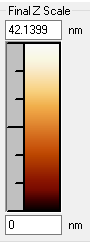
\includegraphics[scale=0.7]{Bilder/Contact_Mode/Rohdaten/try1_scalebar.PNG}
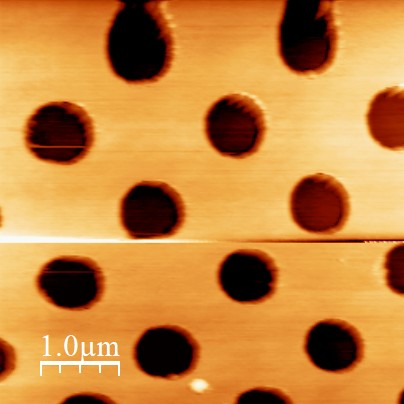
\includegraphics[scale=0.5]{Bilder/Contact_Mode/Rohdaten/try1.JPG}
\caption{Image from the sample recorded in contact mode.}
\label{fig:Contact_raw_data}
\end{figure}

\begin{table}[h]
\centering
\begin{tabular}{|c|c|c|}
\hline 
h$_1$ & h$_2$ & h$_3$ \\ 
\hline 
\SI{25.74 \pm 1.01}{nm} & \SI{25.88 \pm 1.01}{nm} & \SI{26.19 \pm 1.01}{nm} \\ 
\hline
h$_4$ & h$_5$ & h$_6$ \\ 
\hline 
\SI{26.00 \pm 1.01}{nm} & \SI{25.74 \pm 1.01}{nm} & \SI{23.13 \pm 1.01}{nm}  \\ 
\hline 
 h$_7$ & h$_8$ &  \\ 
\hline 
\SI{24.07\pm 1.01}{nm} & \SI{25.11 \pm 1.01}{nm} &  \\ 
\hline 
\end{tabular} 
\caption{Measured height for the structures in contact mode.}
\label{tab:Contact_height}
\end{table}

Fig. \ref{fig:Contact_raw_data} shows the measured image from the sample in contact mode. The height profiles are extracted from a straight line approximately through the center of the circles. \\
The measurement for the heights are listed in Tab. \ref{tab:Contact_height}. The height measurement therefor yield the following result:
\begin{equation*}
h_{measured}^{contact} = \SI{25.23 \pm 1.08}{nm}
\end{equation*}
With this the calibration constant can be calculated:
\begin{equation*}
k_z^{contact} = 0.75297 \pm 0.08560
\end{equation*}

\begin{figure}
\centering
\includegraphics[scale=0.5]{Bilder/Contact_Mode/Snap_in_curve.PNG}
\caption{Snap-in curve measured in contact mode.}
\label{fig:Contact_snap_in}
\end{figure}

Fig. \ref{fig:Contact_snap_in} shows the snap-in curve measured with the setup used in the contact mode. The linear fit yields the averaged slope for the linear regime:
\begin{equation*}
|\alpha| = \SI{0.627 \pm 0.023}{V \per \mu m}
\end{equation*}
With this one calculates the force-calibration constant as:
\begin{equation*}
k_F^{contact} = (2.16 \pm 0.25 \, (stat.) \, _{+ 0.77} ^{- 0.42} \, (sys.)) \times 10^{-10} \si{N \per mV}
\end{equation*}

By determing the difference $\Delta _{adhesion}$ between the T-B Signal at the constant part and at the lowest point in the snap-in curve (fig. \ref{fig:Contact_snap_in}) one can calculate the adhesion force as:
\begin{equation*}
F_{adhesion} = \Delta _{adhesion} \cdot k_F^{contact}
\end{equation*}
The result is:
\begin{equation*}
F_{adhesion} = (1.43140 \pm 0.00023 \, (stat.) \, _{+ 0.50783} ^{- 0.28057} \, (sys.)) \times 10^{-8} \si{N}
\end{equation*}
The load force, meaning the force with which the tip is pressed onto the sample, can be calculated with the difference $\Delta _{load}$ between the T-B signal at the two points with $Z=0$ in the snap-in curve (fig. \ref{fig:Contact_snap_in}) as:
\begin{equation*}
F_{load} = \Delta _{load} \cdot k_F^{contact}
\end{equation*}
The result is:
\begin{equation*}
F_{load} = (5.68 \pm 0.19 \, (stat.) \, _{+ 2.01} ^{- 1.11} \, (sys.)) \times 10^{-9} \si{N}
\end{equation*}


\subsection{Tapping Mode}

\begin{figure}
\centering
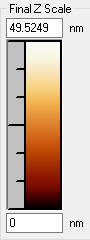
\includegraphics[scale=0.7]{Bilder/Tapping_Mode/Rohdaten/try3_scalebar.PNG}
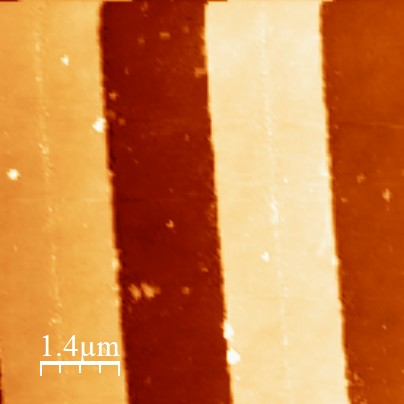
\includegraphics[scale=0.5]{Bilder/Tapping_Mode/Rohdaten/try3.JPG}
\caption{Image from the sample recorded in tapping mode.}
\label{fig:Tapping_raw_data}
\end{figure}

\begin{table}[h]
\centering
\begin{tabular}{|c|c|c|}
\hline 
h$_1$ & h$_2$ & h$_3$ \\ 
\hline 
\SI{27.13 \pm 0.39}{nm} & \SI{27.79 \pm 0.39}{nm} & \SI{26.90 \pm 0.39}{nm}  \\ 
\hline 
h$_4$ & h$_5$ & h$_6$ \\ 
\hline 
\SI{27.07 \pm 0.39}{nm} & \SI{27.09 \pm 0.39}{nm} & \SI{27.47 \pm 0.39}{nm}  \\ 
\hline 
 h$_7$ & & \\ 
\hline 
\SI{28.02 \pm 0.39}{nm} & &  \\ 
\hline 
\end{tabular} 
\caption{Measured height for the structures in tapping mode.}
\label{tab:Tapping_height}
\end{table}

Fig. \ref{fig:Tapping_raw_data} shows the mesured image from the sample in tapping mode. This looks different as in contact mode, because its an other area from an identical sample. The height profiles are extracted as straight lines perpendicular to the lines on the sample. \\
The measurement for the heights are listed in Tab. \ref{tab:Contact_height}. The height measurement therefor yield the following result:
\begin{equation*}
h_{measured}^{tapping} = \SI{27.35 \pm 0.42}{nm}
\end{equation*}
With this the calibration constant can be calculated:
\begin{equation*}
k_z^{tapping} = 0.695 \pm 0.074
\end{equation*}

\begin{figure}
\centering
\includegraphics[scale=0.5]{Bilder/Tapping_Mode/Snap_in_curve.PNG}
\caption{Measured amplitude plotted against the sample-tip distance.}
\label{fig:Tapping_snap_in}
\end{figure}

Fig. \ref{fig:Tapping_snap_in} shows the measured amplitude plotted against the sample-tip distance with the setup used in the tapping mode. The linear fit yields the averaged slope for the linear regime:
\begin{equation*} 
|\alpha| = \SI{1.6330 \pm 0.0057}{V \per \mu m}
\end{equation*}
With this one calculates the force-calibration constant as:
\begin{equation*}
k_F^{tapping} = (1.70 \pm 0.18 \, (stat.) \, _{+ 0.49} ^{- 0.25} \, (sys.)) \times 10^{-5} \si{N \per mV}
\end{equation*} \\

\subsection{Magnetic Microscopy}



\section{Discussion}
$k_F^{contact}$ is several magnitudes of order smaller than $k_F^{tapping}$. As the voltage can be measured with the same certainty this means that in contact mode the resolution with which the the force on the cantilever can be measured is much higher than in tapping mode. This makes sense as the forces to be measured in cantact mode are smaller than those in tapping mode. \\
The statistical error on the force calibration constants is about 10\%. The systematical error only due to the error on the known force constant of the cantilever is with up to 35\% much higher. 








\bibliography{AFM}% Produces the bibliography via BibTeX.

\end{document}
